\documentclass[12pt,a4paper,openright,twoside]{book}
\usepackage[utf8]{inputenc}
\usepackage{float}

\newcommand{\thesislang}{italian}
\usepackage{thesis-style}
% version
\newcommand{\versionmajor}{0}
\newcommand{\versionminor}{1}
\newcommand{\versionpatch}{2}
\newcommand{\version}{\versionmajor.\versionminor.\versionpatch}
\typeout{Document version: \version}

\begin{document}

\frontmatter

% ! TeX root = thesis-main.tex
\title{Title}
\author{Candidate Name Here}
\date{\today}

\newgeometry{margin=0.8in}
\begin{titlepage}
	\begin{center}
		% \vspace*{0.2cm}

		\Huge
		\vspace{4cm}
		\textbf{
			ChEBI
			\\
			Chemical Entities of Biological Interest
		}

		\large
		\vspace{1cm}
		Elaborato in
		\\
		\textsc{Web Semantico}

		\vspace{5.5cm}
		\begin{minipage}[t]{0.64\textwidth}
			\begin{flushleft}
				\textit{Leonardo Micelli}
				\\
				\textbf{leonardo.micelli@studio.unibo.it}
				\\
				\textbf{0001031320}
				\\
				\vspace{0.4cm}
				\textit{Filippo Vissani}
				\\
				\textbf{filippo.vissani@studio.unibo.it}
				\\
				\textbf{0001026702}
			\end{flushleft}
		\end{minipage}

		\vfill
		\noindent\hrulefill
		\vspace{0.3cm}
		\Large
		\\
		Anno Accademico 2022-2023
	\end{center}
\end{titlepage}
\restoregeometry


%----------------------------------------------------------------------------------------
\tableofcontents
%----------------------------------------------------------------------------------------

\mainmatter

%----------------------------------------------------------------------------------------
\chapter{\introductionname}
\label{chap:introduction}
%----------------------------------------------------------------------------------------

ChEBI (Chemical Entities of Biological Interest) è un'ontologia completa di entità chimiche, con particolare attenzione a quelle di rilevanza biologica. ChEBI è progettato per essere utilizzato nell'annotazione e nell'indicizzazione di composti chimici in database e letteratura, nonché nell'analisi di dati chimici.
L'ontologia ChEBI fornisce una classificazione gerarchica delle entità chimiche, basata sulle loro proprietà strutturali e funzionali, nonché sui loro ruoli e applicazioni biologiche. L'ontologia comprende varie classi di composti, come aminoacidi, nucleotidi, lipidi, carboidrati, steroidi e prodotti naturali, nonché composti sintetici e farmaci.
ChEBI contiene informazioni estese sulle proprietà e le attività delle entità chimiche, tra cui le loro strutture chimiche, i pesi molecolari, i punti di fusione, i punti di ebollizione, le solubilità e gli effetti farmacologici.

%----------------------------------------------------------------------------------------
\chapter{Panoramica di ChEBI} % or Background
\label{chap:panoramica}
%----------------------------------------------------------------------------------------
La struttura di ChEBI è quella di un grafico direzionato aciclico (DAG),
differenziandosi da una semplice tassonomia nel fatto che un nodo figlio può avere più padri.

\begin{figure}[H]
	\centering
	\includegraphics[width=\linewidth]{figures/caffeine.png}
	\caption{Struttura DAG di ChEBI}
	\label{fig:Caffeine}
\end{figure}

L'ontologia è a sua volta suddivisa in tre sotto-ontologie principali, chiamate Chemical Entity, Role e Subatomic Particle.

\section{Chemical Entity}

Una \textit{Chemical Entity} è definita come qualsiasi entità molecolare, sia essa sintetica o di origine naturale, che ha una struttura chimica ben definita ed è in grado di interagire con i sistemi biologici.

In ChEBI, i le entità chimiche sono suddivise in quattro sotto-categorie principali:
\begin{itemize}
	\item \textit{Group}: è un insieme di entità chimiche che hanno una struttura chimica comune.
	\item \textit{Molecular Entity}: è un insieme di atomi che sono legati tra loro da legami chimici.
	\item \textit{Atom}: è l'unità minima di materia che non può essere ulteriormente divisa senza perdita di identità.
	\item \textit{Chemical Substance}: è una sostanza chimica che ha una composizione chimica ben definita.
\end{itemize}


\begin{figure}[H]
	\centering
	\includegraphics[width=\linewidth]{figures/chemical-entity.png}
	\caption{Gerarchia più esterna di chemical entity}
	\label{fig:ChemicalEntity}
\end{figure}
\section{Role}
Un \textit{Role} è una funzione o un compito che una entità chimica può svolgere. Un ruolo può essere svolto da una singola entità chimica o da un gruppo di entità chimiche. In ChEBI, i ruoli sono suddivisi in tre sotto-categorie principali:
\begin{itemize}
	\item \textit{Biological Role}: è un ruolo che una entità chimica può svolgere in un organismo vivente.
	\item \textit{Chemical Role}: è un ruolo che una entità chimica può svolgere in un composto chimico.
	\item \textit{Application}: è un ruolo che una entità chimica può svolgere in un processo industriale o in un'attività umana.
\end{itemize}

\begin{figure}[H]
	\centering
	\includegraphics[width=\linewidth]{figures/role.png}
	\caption{Gerarchia più esterna di role}
	\label{fig:Role}
\end{figure}

\section{Subatomic Particle}
Una \textit{Subatomic Particle} è una particella più piccola di un atomo.
In ChEBI, le particelle subatomiche sono suddivise nelle seguenti sotto-categorie principali:
\begin{itemize}
	\item \textit{Boson}: è una particella subatomica responsabile delle interazioni fondamentali e del fenomeno della massa.
	\item \textit{Composite Particle}: è una particella subatomica che è costituita da più di un quark.
	\item \textit{Fermion}: è una particella subatomica che ha una massa non nulla e che interagisce solo con altre particelle subatomiche.
	\item \textit{Fundamental Particle}: è una particella subatomica che non può essere ulteriormente divisa senza perdita di identità.
	\item \textit{Nuclear Particle}: è una particella subatomica che costituisce il nucle di un atomo.
\end{itemize}

\begin{figure}[H]
	\centering
	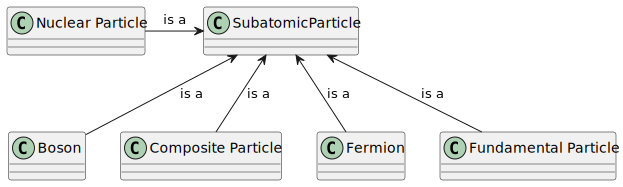
\includegraphics[width=\linewidth]{figures/subatomic-particle.png}
	\caption{Gerarchia più esterna di subatomic particle}
	\label{fig:SubatomicParticle}
\end{figure}

%----------------------------------------------------------------------------------------
\chapter{Esempi di Classi}
\label{chap:classexamples}

\begin{figure}[H]
	\centering
	\includegraphics[width=\linewidth]{figures/class.png}
	\caption{Esempio di classe}
	\label{fig:Class}
\end{figure}

\lstinputlisting[
	float,
	language=XML,
	caption={OWL class for caffeine},
	label={lst:caffeine},
]{listings/caffeine.xml}

%----------------------------------------------------------------------------------------
\chapter{Mapping} % possible chapter for Projects
\label{chap:mapping}
%----------------------------------------------------------------------------------------

%----------------------------------------------------------------------------------------
\chapter{Estensioni} % possible chapter for Projects
\label{chap:extensions}
%----------------------------------------------------------------------------------------

%----------------------------------------------------------------------------------------
\chapter{Progetti} % possible chapter for Projects
\label{chap:projects}
%----------------------------------------------------------------------------------------

%----------------------------------------------------------------------------------------
\chapter{Conclusioni}
\label{chap:conclusions}
%----------------------------------------------------------------------------------------


%----------------------------------------------------------------------------------------
% BIBLIOGRAPHY
%----------------------------------------------------------------------------------------

%\nocite{*} % uncomment this to show all the reference in the .bib file
\bibliographystyle{plain}
\bibliography{bibliography}


\end{document}